In order to more fully understand and appreciate the process of extracting the 3D kinematics of total knee arthroplasty components from single-plane digital images, we must first explore the basics of computer vision. Specifically, the elements of image formation of and object projection.

\subsection{Geometric Transformations}
\label{sec:geometric-transformations}
Geometric primitives, such as points, are fundamental building blocks for representing shapes and objects in computer graphics. In this section, we will discuss how points can be represented in 2D and 3D space..

\subsubsection{2D and 3D Points}
\label{sec:geometric-points}
In N-dimensional space, a point is represented as a set of N scalars, each representing a magnitude in a particular direction. This can be represented mathematically as a column vector (\cref{eq:point}). In two dimensions, a point is represented with two elements, $\mathbf{x} = [x , y]^{T}$. Similarly, in three dimensions, a point is represented with three elements, $\mathbf{x} = [x , y , z]^{T}$.

\begin{equation}
    \mathbf{x} = \begin{bmatrix}
        x_1 \\ x_2 \\ \vdots \\ x_{N-1} \\ x_N
    \end{bmatrix} \in \mathbb{R}^N
    \label{eq:point}
\end{equation}

Homogeneous coordinates provide a way to represent points with an additional scale factor, $\tilde{w}$. This allows us to perform rotations and translations simultaneously and successively using matrix multiplications. Homogeneous coordinates for a point in N-dimensional space are represented as a column vector with N+1 elements (\cref{eq:homog-point}. In most model-image registration applications, the scale factor $\tilde{w}$ is set to 1. When dealing with homogenous coordinates, $\mathbf{\tilde{x}} = \tilde{w}\mathbf{\bar{x}}$, where $\mathbf{\tilde{x}}$ is the scaled version of $\bar{\mathbf{x}}$, and $\bar{\mathbf{x}}$ is simply the original vector, $\mathbf{x}$ with a $1$ appended.

\begin{equation}
    \tilde{\mathbf{x}} = \begin{bmatrix}
        \tilde{x_1} \\ \tilde{x_2} \\ \vdots \\ \tilde{x_N} \\ \tilde{w}
    \end{bmatrix} = \tilde{w}\begin{bmatrix}
        \mathbf{x}\\ 1
    \end{bmatrix} = \tilde{w}\bar{\mathbf{x}}
    \label{eq:homog-point}
\end{equation}

\subsubsection{2D Transformations}
\label{sec:2d-transformations}
Transformations are operations that change the position, orientation, or shape of an object in 2D space. One of the most basic transformations is a translation, which moves an object by adding a displacement vector to its position (\cref{eq:translation}).

\begin{equation}
    \begin{aligned}
        \mathbf{x'} &= \begin{bmatrix}
            x  \\ y 
        \end{bmatrix} + \begin{bmatrix}
            t_x \\ t_y
        \end{bmatrix} = \mathbf{x} + \begin{bmatrix}
            t_x \\ t_y
        \end{bmatrix} = \mathbf{x} + \mathbf{t}\\
        &\text{Or, using homogeneous coordinates and matrix multiplication} \\
        &= \begin{bmatrix}
            1 & 0 & t_x \\ 0 & 1 & t_y
        \end{bmatrix} \begin{bmatrix}
            x \\ y \\ 1
        \end{bmatrix} = \begin{bmatrix}
            \mathbf{I} & \mathbf{t}
        \end{bmatrix}\bar{\mathbf{x}} \\
    \end{aligned}
    \label{eq:translation}
\end{equation}

In this equation, $\mathbf{x}$ is the original position of the object, $\mathbf{x'}$ is the transformed position, and $\mathbf{t}$ is the displacement vector that specifies the amount of translation in the $x$ and $y$ directions. Using homogeneous coordinates and matrix multiplication allows for the convenient representation of multiple transformations as a single matrix multiplication, as well as for the composition of multiple transformations (\cref{eq:mult-translation}).

\begin{equation}
    \begin{aligned}
        \mathbf{\bar{x}}'' &= \begin{bmatrix}
            1 & 0 & t_x \\ 0 & 1 & t_y \\ 0 & 0 & 1
        \end{bmatrix} 
        \begin{bmatrix}
            1 & 0 & q_x \\ 0 & 1 & q_y \\ 0 & 0 & 1
        \end{bmatrix} \begin{bmatrix}
            x \\ y \\ 1 
        \end{bmatrix}\\
        &= \begin{bmatrix}
            x + t_x + q_x \\ y + t_y + q_y \\ 1
        \end{bmatrix}
    \end{aligned}
    \label{eq:mult-translation}
\end{equation}

The next type of 2D transformation is a rotation, which changes the orientation of an object, but not its shape (Eq. \ref{eq:2d-rot}, \ref{eq:2d-rot-mat}). 

\begin{equation}
    \begin{aligned}
        \mathbf{x}' = \mathbf{Rx}
    \end{aligned}
    \label{eq:2d-rot}
\end{equation}

where
\begin{equation}
    \mathbf{R} = \begin{bmatrix}
        cos\theta & -sin \theta \\ sin \theta & cos \theta 
    \end{bmatrix}
    \label{eq:2d-rot-mat}
\end{equation}

This will rotate an object $\theta$ in the counter clockwise direction. 

It's also possible to perform a rotation and a translation at the same time, by replacing the identity matrix $\mathbf{I}$ in Equation \ref{eq:translation} with the rotation matrix $\mathbf{R}$ from Equation \ref{eq:2d-rot-mat}. This results in the transformation shown in Equation \ref{eq:2d-rot-trans}. This transformation preserves lengths and angles.

\begin{equation}
    \mathbf{x}' = \begin{bmatrix}
        \mathbf{R}_{2 \times 2} & \mathbf{t}
    \end{bmatrix} \bar{\mathbf{x}}
    \label{eq:2d-rot-trans}
\end{equation}


A scaled rotation will change the size of the object by some scaler factor, $s$ (Eq. \ref{eq:2d-scaled-rot}); this transformation preserves angles.

\begin{equation}
    \mathbf{x}' = \begin{bmatrix}
        s\mathbf{R}_{2 \times 2} & \mathbf{t}
    \end{bmatrix}\bar{\mathbf{x}}
    \label{eq:2d-scaled-rot}
\end{equation}

An affine transformation preserves parallelism, and is simply a pre-multiplication by an arbitrary $2 \times 3$ matrix (Eq. \ref{eq:2d-affine}).

\begin{equation}
    \begin{aligned}
        \mathbf{x}' &= \mathbf{A\bar{x}}\\
        &\text{where}\\
        \mathbf{A} &= \begin{bmatrix}
            a_{11} & a_{12} & a_{13} \\ a_{21} & a_{22} & a_{23}
        \end{bmatrix}
    \end{aligned}
    \label{eq:2d-affine}
\end{equation}

A projection matrix (or perspective transformation) is one that operates on homogeneous coordinates (Eq. \ref{eq:2d-projection}).

\begin{equation}
    \begin{aligned}
        \tilde{\mathbf{x}}' &= \tilde{\mathbf{H}}\tilde{\mathbf{x}}\\
    \end{aligned}
    \label{eq:2d-projection}
\end{equation}

To obtain inhomogeneous results, the resultant $\tilde{\mathbf{x}}'$ must be normalized (Eq. \ref{eq:2d-homog-norm}). A projective transformation preserves straight lines.

\begin{equation}
    \begin{aligned}
        x'&= \frac{\tilde{x}}{\tilde{w}}  &  y' &= \frac{\tilde{y}}{\tilde{w}}\\
        &= \frac{h_{11}x + h_{12}y + h_{13}}{h_{31}x + h_{32}y + h_{33}} &  &= \frac{h_{21}x + h_{22}y + h_{23}}{h_{31}x + h_{32}y + h_{33}}
    \end{aligned}
    \label{eq:2d-homog-norm}
\end{equation}

\subsubsection{3D Transformations}
\label{sec:3d-transformations}

3D transformations operate on 3D points (Eq. \ref{eq:point}) in a similar way to 2D transformations. In general, all types of transformations, including translations, rotations, scaled rotations, and projections, can be represented by matrices in 3D space, with the only difference being that the dimensions are increased by one.

One aspect of 3D rotations that adds complexity is the possibility of multiple axes of rotation. This introduces the issue of non-commutativity, which means that the order in which rotations are applied matters. To handle this, we can use the concept of Euler angles, which represent the rotations as composite rotations about canonical axes. These rotations are represented by matrices (Eq. \ref{eq:euler-angles}). Note that these matrices are post-multiplied by each other to determine the final rotation matrix for object-centered rotations. Additionally, given a rotation matrix and the corresponding Euler rotations, it is possible to decompose the matrix into its composite rotations about the canonical axes.

\begin{equation}
    \begin{aligned}
        R_{x} &= \begin{bmatrix}
            1 & 0 & 0 \\ 0 & c_x & -s_x \\ 0 & s_x & c_x
        \end{bmatrix}
        &R_{y} &= \begin{bmatrix}
            c_y & 0 & s_y \\ 0 & 1 & 0 \\ -s_y & 0 & c_y
        \end{bmatrix}
        &R_{z} &= \begin{bmatrix}
            c_z & -s_z & 0 \\ s_z & c_z & 0 \\ 0 & 0 & 1
        \end{bmatrix} \\
    \end{aligned}
    \label{eq:euler-angles}
\end{equation}


\paragraph*{3D to 2D Projections}
Geometric primitives, such as points, lines, and polygons, are the building blocks of computer graphics. These basic shapes can be transformed and combined in various ways to create more complex objects and scenes. In order to represent these 3D primitives and objects in 2D image space, we must apply transformations that manipulate their position, orientation, and other properties. By using these transformations, we can create the illusion of depth and spatial relationships on a flat display. Understanding how to work with primitives and transform them is crucial for creating a wide range of visual effects and graphics in computer graphics.

In computer graphics, one of the most basic methods of projecting three-dimensional objects onto a two-dimensional image plane is an orthographic projection. This projection simply drops the depth component of the object and flattens it onto the image plane (Eq. \ref{eq:orthographic-proj}. This can be thought of as mimicking a camera with a long focal length, or when the depth of the object is shallow compared to its distance from the camera (also known as a weak perspective projection). In this equation, $\mathbf{p}$ represents a point in 3D space and $\mathbf{x}$ represents the projected point in 2D image space.

\begin{equation}
    \tilde{\mathbf{x}} = \begin{bmatrix}
        1 & 0 & 0 & 0 \\ 0 & 1 & 0 & 0 \\ 0 & 0 & 0 & 1
    \end{bmatrix}\tilde{\mathbf{p}}
    \label{eq:orthographic-proj}
\end{equation}

Perspective projection 
The most common 3D-2D projection is \emph{perspective projeciton}, which mimics how human's normally see by taking depth-perception into account. This can be done by scaling each point by it's $z$ position relative to the camera (Eq. \ref{eq:perspective-proj}). We can also perform this using homogeneous coordinates (Eq. \ref{eq:perspective-matrix}).

\begin{equation}
    \bar{\mathbf{x}} = \mathcal{P}_z(\mathbf{p}) = \begin{bmatrix}
        x/z \\ y/z \\ 1
    \end{bmatrix}
    \label{eq:perspective-proj}
\end{equation}

\begin{equation}
    \tilde{\mathbf{x}} = \begin{bmatrix}
        1 & 0 & 0 & 0 \\ 0 & 1 & 0 & 0 \\ 0 & 0 & 1 & 0 
    \end{bmatrix}\tilde{\mathbf{p}}
    \label{eq:perspective-matrix}
\end{equation}

The perspective projection is the cornerstone of model-image registration. If a matrix can be created that mimics the fluoroscopic imaging setup in the clinic, then this offers a strong possibility of re-creating a virtual scene with the same geometry as the actual scene.

\subsection{Image Formation and Camera Properties}
\label{sec:img-form-camera-props}
Utilizing the knowledge of geometric transformations and projective geometries, a model of a camera can be systematically constructed step by step.
The reference frame is standardized, with the $z$ direction along the focal direction of the camera, the $x$ direction to the right, and the $y$ direction such that the right-hand rule is maintained.
The origin is at the center of the camera.

The object of interest is described as a collection of points, $\mathbf{p}_i =  [x_i, y_i, z_i, 1] \text{ for } i = 1,2,\cdots,N$.
In practice, all operations are uniformly performed on all points.
For clarity, the subsequent equations will illustrate the process using a single point of the object.

The first step is describing the location and orientation of the object with respect to the camera.
This rotation and translation can be captured using a single 3D homogeneous transformation matrix (\cref{eq:4x4-homog-transformation}).

\begin{equation}
    \tilde{\mathbf{p}}' = \begin{bmatrix}
        \mathbf{R}_{3 \times 3} & \mathbf{t}_{3 \times 1} \\ \mathbf{0}_{1 \times 3} & 1
    \end{bmatrix} \tilde{\mathbf{p}}
    \label{eq:4x4-homog-transformation}
\end{equation}

Then, a projective transform is applied to each point in the object, controlling for the relative size and scaling based on the focal distance.
Geometrically, this relationship can be visualized with similar triangles (\cref{fig:perspective-projection}) and quantified using the ratio of lengths (\cref{eq:perspective-projection}).
In these equations, $f'$ is the focal distance in units of length.

\begin{figure}[h!]
    \begin{center}
        \includegraphics[width=0.85\linewidth]{figs/background/png/perspective-projection.png}
    \end{center}
    \caption{The geometry of perspective projection can be visualized by using similar triangles. The overall scaling of the image is based on the ratio of the focal length to the depth of the object.                                                 }
    \label{fig:perspective-projection}
\end{figure}


\begin{equation}
    \begin{aligned}
        \tilde{\mathbf{x}}_{i} &= \begin{bmatrix}
            f' & 0 & 0 \\ 0 & f' & 0 \\ 0 & 0 & 1 
        \end{bmatrix} \tilde{\mathbf{p}}' \\
        &\text{where} \\
        x_i &= p_x'\frac{f'}{p_z'} \\
        y_i &= p_y'\frac{f'}{p_z'} \\
    \end{aligned}
    \label{eq:perspective-projection}
\end{equation}

The standard image reference frame places the origin at the top left corner of the image, with the positive x-direction to the right, and the positive y-direction down.
This introduces the idea of the principal point, $(c_x,c_y)$, which is the location where the optical axis of the camera intersects the image plane perpendicularly.
In the camera model, the principal point is a translation starting at the image plane's origin (Eq. \ref{eq:principal-point}).



\begin{equation}
    \begin{aligned}
        \tilde{\mathbf{x}}_{i} &= \begin{bmatrix}
            f' & 0 & c_x \\ 0 & f' & c_y \\ 0 & 0 & 1 
        \end{bmatrix} \tilde{\mathbf{p}}' \\
        &\text{where} \\
        c_x &\approx \frac{W_{image}}{2} \\
        c_y &\approx \frac{H_{image}}{2} \\
    \end{aligned}
    \label{eq:principal-point}
\end{equation}


Lastly, the image coordinates, $\tilde{\mathbf{x}}_{i}$ must be converted to pixel coordinates using the pixel scaling factor.
The pixel scale factor is defined by the parameters $k_x$ and $k_y$, which represent the number of pixels per unit distance in the x and y directions, respectively.
Multiplying the perspective projection matrix by the pixel scale factor yields a new matrix that maps 3D points in ``world coordinates'' directly to pixel coordinates in the image.
\begin{equation}
    \begin{aligned}
        \tilde{\mathbf{x}}_{pix} &= \begin{bmatrix}
            k_x & 0& 0 \\ 0 & k_y & 0 \\ 0 & 0 & 1
        \end{bmatrix} \begin{bmatrix}
            f' & 0 & c_x \\ 0 & f' & c_y \\ 0 & 0 & 1 
        \end{bmatrix}\tilde{\mathbf{p}}' \\
        & = \begin{bmatrix}
            f_x & 0 & c_x \\ 0 & f_y & c_y \\ 0 & 0 & 1 
        \end{bmatrix}\tilde{\mathbf{p}}'\\
        &\text{where}\\
        f_x &= k_x f' \text{        and        } f_y = k_y f' \\
        &\text{Are focal distances in units of pixels} 
    \end{aligned}
    \label{eq:pixel-scaling}
\end{equation}


To generate a simple binary rasterization of the image, the space between projected points is interpolated and filled in, resulting in a binary ``shadow'' of the object on the image plane.
While more comprehensive image formation entails coloring, shading, and ray tracing, such complexity is unnecessary for the purpose of model-image registration of implant geometries in fluoroscopic images, and thus will not be addressed.

%%% Local Variables:
%%% mode: latex
%%% TeX-master: "../../../Andrew_Jensen_Dissertation"
%%% End:


\subsection{Image Processing}
\label{sec:image-processing}
Digital image processing is a field of computer vision that deals with the manipulation, analysis, and interpretation of digital images.
It focuses on algorithms and techniques that extract meaningful information from images and enhance visual quality.
We can leverage these algorithms to efficiently and autonomously extract information relevant to model-image registration.

\subsubsection{Filtering and convolution}
\label{sec:filtering-convolution}
As previously discussed, image formation yields a collection of 2D points, $\mathbf{x}_{pix}$.
We can write the intensity values at each pixel location as a digital signal, $f(\mathbf{x}_{pix}) = f(i,j)$, where $(i,j)$ represents the pixel locations in the image, and the function returns the intensity value.
We can then use standard methods of digital signal processing in order to extract meaningful information from images.

The most widely used filter is a linear filter \cite{szeliskiComputerVisionAlgorithms2022}, where the output is some linear operation on the neighboring pixels (\cref{eq:convolution}).
This process is known as a \emph{convolution}.
In a convolution, the kernel, $h$, is shifted along the input image, $f$, and the resultant image, $g$, is the dot product of those two matrices at that specific location.

\begin{equation}
    \begin{aligned}
        g(i,j) &= \sum_{k,l}f(i-k,j-l)h(k,l) \\
        &= \sum_{k,l}f(k,l)h(i-k,j-l) \\
        &\text{Where we use the following notation}\\
        g&= f * h
    \end{aligned}
    \label{eq:convolution}
\end{equation}

The convolution operation is \emph{linear shift invariant}, which means that it obeys the superposition principle (\cref{eq:superposition}) and the shift invariance principle (\cref{eq:shift-invariance}).
This is a powerful property, because it will behave the same everywhere on the input signal/image (e.g. an edge detector will detect an edge, no matter where the edge is on the input image).

\begin{equation}
    h *(f + g) = h*f + h*g
    \label{eq:superposition}
\end{equation}

\begin{equation}
    g(i,j) = f(i+k,j+l) \Longleftrightarrow (h*g)(i,j) = (h*f)(i+k,j+l)
    \label{eq:shift-invariance}
\end{equation}

A common filter applied to images is the Gaussian kernel (\cref{eq:gaussian-kernel}).
This kernel is shaped as a 2D discrete Gaussian, and has the effect of blurring an image and removing noise.

\begin{equation}
    \text{Gaussian filter}=\frac{1}{256}\begin{bmatrix}
        1 & 4 & 6 & 4 & 1 \\
        4 & 16 & 24 & 16 & 4\\
        6 & 24 & 36 & 24 & 6\\
        4 & 16 & 24 & 16 & 4\\
        1 & 4 & 6 & 4 & 1 \\
    \end{bmatrix}
    \label{eq:gaussian-kernel}
\end{equation}

Another is the box kernel, which averages the value of the nearest K pixels (\cref{eq:box-filter}).

\begin{equation}
    \text{Box filter} = \frac{1}{K^{2}}\begin{bmatrix}
        1 & 1 & \cdots &1\\
        1 & 1 & \cdots &1 \\
        \vdots & \vdots & 1 & \vdots \\
        1 & 1 & \cdots & 1
    \end{bmatrix}
    \label{eq:box-filter}
\end{equation}

Edge filters can also be created to detect vertical (\cref{eq:vert-edge-filter}), horizontal (\cref{eq:horiz-edge-filter}), or diagonal edges (\cref{eq:diag-edge-filter}).
As each of the filters moves across the feature it is designed for, that region of the output will be more highly activated than other regions, extracting out the desired components.
The orientation of each of these filters can be hand-selected to find desirable attributes in images.

\begin{equation}
    \text{vertical edge filter} = \begin{bmatrix}
            0 & 1 & 0 \\
            0 & 1 & 0 \\
            0 & 1 & 0 \\
    \end{bmatrix}
    \label{eq:vert-edge-filter}
\end{equation}

\begin{equation}
    \text{horizontal edge filter} =\begin{bmatrix}
        0 & 0 & 0 \\
        1 & 1 & 1 \\
        0 & 0 & 0 \\
    \end{bmatrix}
    \label{eq:horiz-edge-filter}
\end{equation}

\begin{equation}
    \begin{aligned}
        \text{diagonal edge filters} = \begin{bmatrix}
            1 & 0 & 0 \\
            0 & 1 & 0\\
            0 & 0 & 1
        \end{bmatrix}& \text{and} & 
        \begin{bmatrix}
            0 & 0 & 1 \\
            0 & 1 & 0\\
            1 & 0 & 0
        \end{bmatrix}
    \end{aligned}
    \label{eq:diag-edge-filter}
\end{equation}

Lastly, we can use a corner filter to find corners in images (\cref{eq:corner-filter}).

\begin{equation}
    \text{Corner filter} = \frac{1}{4}\begin{bmatrix}
        1 & -2 & 1 \\
        -2 & 4 & -2 \\
        1 & -2 & 1 \\
    \end{bmatrix}
    \label{eq:corner-filter}
\end{equation}

Entire subfields of computer vision and image analysis are devoted to creating increasingly useful and complex filters, or collections of filters. These include steerable filters, which determine information occurring in arbitrary directions \cite{freemanSteerableFiltersLocal1992}, recursive filtering \cite{nielsenRegularizationScalespaceEdge1996}, and non-linear filtering \cite{tomasiBilateralFilteringGray1998}.

\subsubsection{Edge detection}
Edge detection is a highly motivated sub-field of image processing in computer vision due to the immense usefulness of algorithmically determining the edges in a given image.
For a human operator, it can be relatively easy to identify edges of interest, but how can this be achieved computationally?
The first approach might be in viewing an image topographically, with regions of different colors and intensity represented by different ``heights''.
Then, an edge simply becomes an area with a steep gradient (\cref{eq:img-grad}).

\begin{equation}
    \begin{aligned}
        \mathbf{J}(\mathbf{x}) = \nabla I(\mathbf{x}) = (\frac{\partial I}{\partial x}, \frac{\partial I}{\partial y})(\mathbf{x})
    \end{aligned}
    \label{eq:img-grad}
\end{equation}

Finding the direction of the steepest ascent/descent at any given location will give us the normal to the local edge at that point. However, the derivative operator will accentuate and amplify high frequencies in the image, causing noise to overpower the signal. Removing the high-frequency information (a low-pass filter) in the image results in gradient detection that is much more aligned with the salient edges of the image. The Gaussian kernel is a good option for an isotropic low-pass filter on a 2D signal (image) (\cref{eq:gauss-kernel-grad})

\begin{equation}
    \begin{aligned}
        \mathbf{J}_{\sigma}(\mathbf{x}) &= \nabla [G_\sigma (\mathbf{x} * I(\mathbf{x}))] \\
        &= \nabla G_\sigma (\mathbf{x}) * I(\mathbf{x}) \\
        &\text{where} \\
        \nabla G_\sigma (\mathbf{x}) &= (\frac{\partial G_{\sigma}}{\partial x}, \frac{\partial G_{\sigma}}{\partial x}) = [-x - y]\frac{1}{\sigma^{2}}\text{exp}(\frac{-(x^2 + y^2)}{2 \sigma^2})
    \end{aligned}
    \label{eq:gauss-kernel-grad}
\end{equation}


A widely-recognized edge detection algorithm was proposed by John Canny in 1986 \cite{cannyComputationalApproachEdge1986}, and utilizes a five-step process.
First, a Gaussian kernel is applied as a low-pass filter (\cref{eq:gauss-kernel-grad}).
Second, directional filters are used to find the gradients in each direction of the image.
Third, a gradient magnitude threshold is applied to remove noise. Fourth, a double threshold is applied to remove both strong and weak edges.
Last, edges are determined from hysteresis. The prevailing limitation of this algorithm is the need to set kernel size and edge-intensity.

\subsubsection{Binary image processing}
\label{sec:binary-img-proc}

A binary image is a digital image that consists only of black and white pixels.
It is often used for labeling or masking an underlying image, where the values of 1 and 0 represent the presence or absence of a particular feature or object.
Binary images are often used in computer vision and image processing applications due to low computational overhead and quick analysis.
They are also useful for storing and transmitting large amounts of data, as the use of only two values reduces the amount of information that needs to be stored and transmitted.

The primary method of processing binary images is morphological, which involves changing the shape of the ``blob'' in order to extract useful information from it.

\begin{figure}[h!]
    \includegraphics[width = \linewidth]{figs/background/png/binary-image-processing.jpg}
    \caption[A collection of morphological operations on a binary image]{A collection of morphological operations on a binary image: (a) original image; (b) dilation; (c) erosion; (d) majority; (e) opening; (f) closing. Image from \cite{szeliskiComputerVisionAlgorithms2022}}
    \label{fig:binary-image-processing}
\end{figure}

Dilation and erosion are the two main operations that are used in model-image registration (\ref{eq:dilation-erosion}).
These functions are each two-fold: first, a convolution operation is applied to the existing binary image, then a threshold is applied to the convolution output to determine if the central pixel is a 0 or 1.
If $f$ is the input image, $s$ is the convolution kernel of $1$s, and $c=f\otimes s$ is the number of $1$s in the convolution output, then dilation and erosion can be expressed in the following way.

\begin{equation}
    \begin{aligned}
        \text{dilate}(f,s) &= \theta(c,1) \\
        \text{erode}(f,s) &= \theta(c,S) 
    \end{aligned}
    \label{eq:dilation-erosion}
\end{equation}

Where $\theta$ represents a thresholding function.

\begin{equation}
    \theta (f,t) = \begin{cases}
        1 &\text{ if } f\ge t \\
        0 &\text{ else}
    \end{cases}
\end{equation}

%%% Local Variables:
%%% mode: latex
%%% TeX-master: "../../../Andrew_Jensen_Dissertation"
%%% End:


\subsection{Image Similarity Metrics}
\label{sec:image-similarity}
One of the key components in model image registration is image similarity.
This fundamentally involves determining how closely the user's synthetic image matches the actual fluoroscopic image.
The choice of similarity metric will be influenced by several key factors, including the a-priori availability of implant/bone geometry and the knowledge of image quality and contrast.
Broadly, there are two classes of image similarity when performing model-image registration: intenisty-based and feature based.

\subsubsection{Intensity Based}
\label{sec:img-sim-intensity}
Intensity based measures are those that utilize specific pixel information in order to determine the difference between two images.
This can be either a global image similarity metric or a measure of specific regions of interest within the image.

A canonical difference between two images would be the p-norm separating them (\cref{eq:p-norm}), which iterates through each pixel of the two images and finds the p-norm difference between each pixel pair.
Common p-norms are the $L_1$ norm (\emph{absolute intensity differences} or \emph{mean absolute difference}) \cite{kanadeStereoMatchingAlgorithm1994} ($p=1$) and the $L_{2}$ norm, or Euclidean norm (\emph{squared intensity differences} or \emph{mean squared difference}) \cite{hannahComputerMatchingAreas1977}($p=2$).

\begin{equation}
    \|A-B\|_{p} = (\sum_{x=0}^{w}\sum_{y=0}^{h}|a_{xy}-b_{xy}|^{p})^{\frac{1}{p}}
    \label{eq:p-norm}
\end{equation}

In Equation \cref{eq:p-norm}, $A$ and $B$ are the two images being compared, $w$ and $h$ are the width and height of the images, and $a_{xy}$ and $b_{xy}$ are the intensity values at pixel $(x,y)$ in the two images, respectively.

While conceptually easy to use, the main limitation of p-norm measures is their lack of spatial information.
For example, an image that has been shifted by a linear transformation would not score well using a p-norm, despite the two images containing only a minor shift, scale, or rotation. One method for overcoming this limitation is to use the cross-correlation, or sliding dot product, between images \cite{bendatRandomDataAnalysis2010,hannahComputerMatchingAreas1977} (\cref{eq:xcorr}).
When used in conjunction with projective geometry, this can help locate regions of interest for a model-based registration pipeline.
The cross-correlation is calculated using the following equation:

\begin{equation}
    \begin{aligned}
        (A \star B)[x,y] &= E[A_{xy} \cdot B_{x + \tau_x,y+\tau_y}] \\
        &= \sum_{\tau_x=-\infty}^{\infty}\sum_{\tau_y=-\inf}^{\infty}a_{xy}b_{x + \tau_x,y + \tau_y}
    \end{aligned}
    \label{eq:xcorr}
\end{equation}

This will determine the regions of each image that are similar, causing the correlation function to ``light up'' at those areas in a similar way to the convolutional operation between two images.
The normalized cross-correlation can also be used (\cref{eq:norm-xcorr}), which removes noise coming from each of the original images.

\begin{equation}
    \begin{aligned}
        \text{normalized cross correlation}(A,B) &= \frac{A \star B}{(A \star A)(B \star B)}
    \end{aligned}\label{eq:norm-xcorr}
\end{equation}

\subsubsection{Feature Based}
\label{sec:img-sim-feature}
Feature based image similarity metrics involve methods for identifying key features in images and using these features to measure differences between two images.
These types of methods almost always involve some type of feature-extraction step, where the various features of interest are calculated and determined for subsequent use.
The two main classes of features are \emph{keypoints} and \emph{edges}.
The simplest method of keypoint detection is using a similar method to intensity-based matching, but having one of the ``images'' as a patch of the desired feature.
With keypoints detected in the input image, one could determine the error of the current pose estimate by taking the Euclidean distance between all image keypoints and all projected keypoints: \cite{burtonAutomaticTrackingHealthy2021} (\cref{eq:kp-error}).
With a-priori information about the keypoints, weights could be assigned to each keypoint in order to emphasize specific regions on the image and the model (\cref{eq:wkp-error})

\begin{equation}
    \begin{aligned}
        \text{Keypoint Error}= (\sum_{i = 0}^{N}(KP_{image,i} - KP_{proj,i})^2)^{\frac{1}{2}}
    \end{aligned}
    \label{eq:kp-error}
\end{equation}

\begin{equation}
    \begin{aligned}
        \text{Weighted Keypoint Error} = (\sum_{i = 0}^{N}w_{i}(KP_{image,i} - KP_{proj,i})^2)^{\frac{1}{2}}
    \end{aligned}
    \label{eq:wkp-error}
\end{equation}

Keypoints are particularly useful when there are invariant features in images and 3D models, like morphological aspects of bones.
However, if these features cannot be detected, alternative measures must be utilized.

\paragraph*{Edges as Features}
Edges are a natural choice of feature when determining image similarity.
Similar to intensity-based image similarity, the similarity between the contours of two images offers a promising metric for determining the overall similarity between two images.
In model-image registration, the contours of the input image and the projected model can easily be compared, which presents a reliable scheme for measuring their similarity.
When the edges are aligned, we say that the model is \textit{properly registered} to the image.
However, how can we determine when the edges are aligned?

As always, the simplest approach is to take the p-norm between the model and image contours (\cref{eq:p-norm}), where instead of taking the difference between the two original images, one is taking the difference of the edges of the images.
This function will be minimized when there is complete overlap between image and model contours.

\paragraph{Drawback of Feature Based Similarity Metrics}
While they can be much more informative and specific, the main drawback of feature based image similarity metrics is the need for feature selection and extraction from the input image.
Historically, this required an immense amount of domain-specific knowledge, and the image processing used to extract those features was often relatively limited in scope.


%%% Local Variables:
%%% mode: latex
%%% TeX-master: "../../../Andrew_Jensen_Dissertation"
%%% End:

